\documentclass[paper=a4, fontsize=11pt]{scrartcl}
\usepackage[T1]{fontenc}
\usepackage[english]{babel}
\usepackage{amsmath,amsfonts,amsthm,mathrsfs}
\usepackage{sectsty} % Allows customizing section commands
\usepackage{listings}
\usepackage{enumitem}
\usepackage{color}
\usepackage{graphicx}
\usepackage{pgf, tikz}

\usetikzlibrary{arrows, automata}

\definecolor{mygreen}{RGB}{28,172,0} % color values Red, Green, Blue
\definecolor{mylilas}{RGB}{170,55,241}
\allsectionsfont{\centering \normalfont\scshape} % Make all sections centered, the default font and small caps
\usepackage{fancyhdr} % Custom headers and footers
\pagestyle{fancyplain} % Makes all pages in the document conform to the custom headers and footers
\fancyhead{} % No page header - if you want one, create it in the same way as the footers below
\fancyfoot[L]{} % Empty left footer
\fancyfoot[C]{} % Empty center footer
\fancyfoot[R]{\thepage} % Page numbering for right footer
\renewcommand{\headrulewidth}{0pt} % Remove header underlines
\renewcommand{\footrulewidth}{0pt} % Remove footer underlines
\setlength{\headheight}{13.6pt} % Customize the height of the header
\numberwithin{equation}{section} % Number equations within sections (i.e. 1.1, 1.2, 2.1, 2.2 instead of 1, 2, 3, 4)
\numberwithin{figure}{section} % Number figures within sections (i.e. 1.1, 1.2, 2.1, 2.2 instead of 1, 2, 3, 4)
\numberwithin{table}{section} % Number tables within sections (i.e. 1.1, 1.2, 2.1, 2.2 instead of 1, 2, 3, 4)
\setlength\parindent{0pt} % Removes all indentation from paragraphs - comment this line for an assignment with lots of text
\newtheorem*{solution}{Solution}

\newcommand{\horrule}[1]{\rule{\linewidth}{#1}} % Create horizontal rule command with 1 argument of height

\title{	
\normalfont \normalsize 
\textsc{Dept. of Computer Science, University of California, Davis\\ECS170 \hspace{.5in}
%%%%%%%%%%%%%%%%%%%%%%%%%%%%
%%%% Add your name here %%%%
%%%%%%%%%%%%%%%%%%%%%%%%%%%%
YOUR NAME - YOUR ID\hspace{.5in} \today}
\horrule{0.5pt} \\[0.4cm]
%%%%%%%%%%%%%%%%%%%%%%%%%%%%%%%%%%%%
%%%% Write the Homework # here %%%%%
%%%%%%%%%%%%%%%%%%%%%%%%%%%%%%%%%%%%
\huge Homework: Search \\
\horrule{2pt} \\[0.5cm]
}

\date{}

\begin{document}

\maketitle

\vspace{-1in}

\section{}
Write down the steps of the open list and closed list for every iteration of the A* algorithm on the weighted
graph below. The start nodes are denoted with S and the goal nodes are denoted with G . The value of the
heuristic is next to each node. Track entries on the open and closed lists with the format discussed in lecture:
<state, f , g , backpointer>

 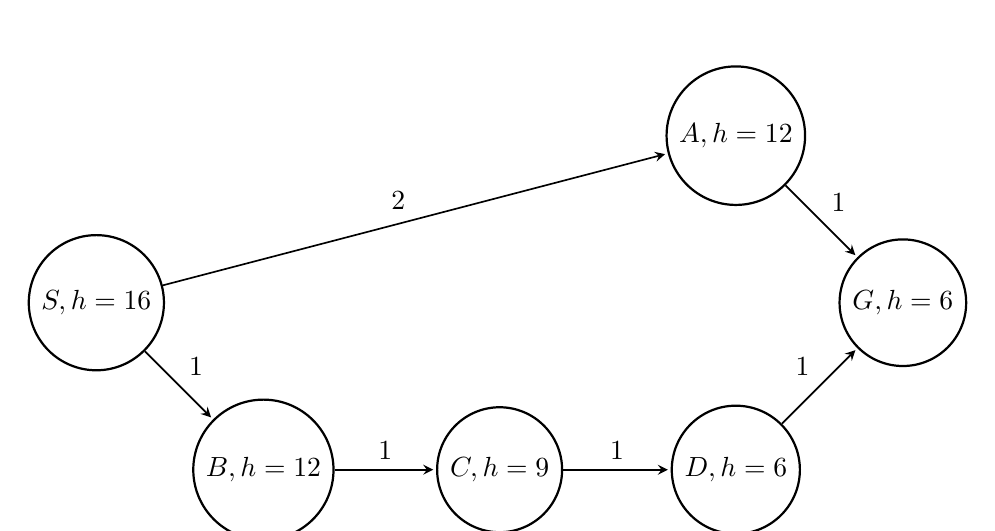
\begin{tikzpicture}[
            > = stealth, % arrow head style
            shorten > = 1pt, % don't touch arrow head to node
            auto,
            node distance = 3cm, % distance between nodes
            semithick % line style
        ]

        \tikzstyle{every state}=[
            draw = black,
            thick,
            fill = white,
            minimum size = 4mm
        ]

        \node[state] (S) {$S, h=16$};
        \node[state] (B) [below right of=S] {$B, h=12$};
        \node[state] (C) [right of=B] {$C, h=9$};
        \node[state] (D) [right of=C] {$D, h=6$};
        \node[state] (G) [above right of=D] {$G, h=6$};
        \node[state] (A) [above left of=G] {$A, h=12$};

        \path[->] (S) edge node {2} (A);
        \path[->] (S) edge node {1} (B);
        \path[->] (B) edge node {1} (C);
        \path[->] (C) edge node {1} (D);
        \path[->] (D) edge node {1} (G);
        \path[->] (A) edge node {1} (G);

    \end{tikzpicture}
   
   
% --- 1 
\begin{center}
 \begin{tabular}{|c|c ||c |c||} 
 \hline
 Open List & - & Closed List & - \\
 \hline
 1 & - & 1 & Empty \\ 
 \hline
 2 & - & 2 & - \\
 \hline
 3 & - & 3 & - \\
 \hline
 4 & - & 4 & - \\
 \hline
 5 & - & 5 & - \\
 \hline
 6 & - & 6 & - \\
 \hline
\end{tabular}
\end{center}

% --- 2
% --- 3
% --- 4
% --- 5
% --- 6
% --- 7
% --- 8
% --- 9
% --- 10
% --- 11
% --- 12

\subsection{}
Why $A^*$ did not find the shortest path in problem 1. How can the problem be fixed?

\section{}
Explain why search is not used for sorting tasks in terms of computational efficiency, task complexity, and
heuristics.

\section{}
There are 255,160 possible unique ways to play the game Tic Tac Toe . To explore some of them, draw the
search tree for starting at the game state below. Label winning states with 2, losing states with 0, and draw
states with 1. You are playing as the O s and it is your turn.

\begin{center}
 \begin{tabular}{|c|c|c|} 
 \hline
 O & X & O \\
 \hline
 - & X & O  \\ 
 \hline
 - & - & X \\
 \hline


\end{tabular}
\end{center}

\subsection{}
Annotate non-terminal search tree nodes with score given by minimax.

\subsection{}
If there are subtrees pruned by alpha-beta minimax, label them as pruned in your search tree.

\subsection{}
What is the best possible outcome for Os and for Xs? What about the worst outcome for each? Are either
likely given if both players used minimax to guide their plays?

\section{}

Given your search subtree for Tic Tac Toe, use UCB1 to find the confidence interval for the subtree. For convenience, here is the UCB1 formula:
\begin{equation}
	\bar{x_i} \pm \sqrt{\frac{2 \ln n}{n_i}}
\end{equation}

\subsection{}
Is MCTS guaranteed to find the best solution in its search? Justify your answer in terms of determinism and stochasticity. If MCTS had fantastically large but finite resources to work with, does the guarantee hold? 

\end{document}